 %!TEX root = coexistence_paper.tex
 \section{Background and System Model}
 We focus on LoRa as an representative LPWAN technologies and handle co-existence for dense LoRa networks with our q-learning framework. In the following sections, we describe the necessary background on LoRa. 
  
 %\subsection{An Overview of SNOW}

 
 %\begin{figure}[!htpb]%{r}{7.3cm}
%\centering\vspace{-0.05in}
%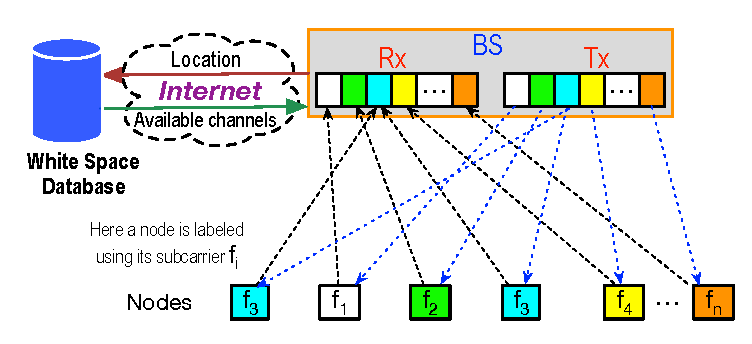
\includegraphics[width=0.44\textwidth]{figs/dual-radio.eps}
%\vspace{-0.1in}
%\caption{\small The SNOW architecture.}
%\label{fig:arch}
%\vspace{-0.1in}
%\end{figure} 
 
 
 %Here we provide a brief overview of the SNOW PHY that we developed previously \cite{snow, snow2, ton_snow}. Its {\bf full description}  is available in~\cite{ton_snow}. Due to long transmission (Tx) range, the nodes in SNOW are directly connected to the BS, forming a star topology as shown in Fig.~\ref{fig:arch}. We use {\bf `node'} to indicate a sensor node.  We assume that the BS knows the locations of the nodes through manual configuration or some existing WSN localization technique~\cite{wsnlocalizationsurvey}. \revise{This assumption is relaxed in our proposed research}. 
%The BS periodically determines white spaces by providing locations of its own and of all other nodes in a cloud-hosted database through the Internet. The BS uses wide white space spectrum as a single wide channel that is split into narrowband orthogonal subcarriers, each of equal spectrum width (bandwidth). Each node has a single half-duplex narrowband radio. It sends/receives on a subcarrier. The nodes are power-constrained, and do not do spectrum sensing or cloud access. As shown in Fig.~\ref{fig:arch}, the BS uses two radios --  one for only transmission (called {\bf\slshape Tx radio})  and the other for only reception (called {\bf\slshape Rx radio}) -- to facilitate concurrent bidirectional communication.  




%
%\begin{figure*}[!htb]
%    \centering\vspace{-0.22in}
%      \subfigure[\footnotesize Node positions in the Detroit metro area\label{fig:outdoor}]{
%	\includegraphics[width=0.37\textwidth]{figs/setup/metro_setup.jpg}
%      }
%    \hfill
%      \subfigure[\footnotesize Uplink reliability\label{fig:reliability_bs_distance}]{
%    \includegraphics[width=0.23\textwidth]{figs/reliability/reliability_bs_distance.eps}
%      }
%      \hfill
%      \subfigure[\footnotesize Distance vs. Tx powers\label{fig:distance_txpower}]{
%        \includegraphics[width=.22\textwidth]{figs/reliability/distance_txpower.eps}
%      }\vspace{-0.2in}
%    \caption{\small Reliability over distances and  varying Tx power.}\vspace{-0.13in}
%    \label{fig:reliability_bs_node}
% \end{figure*}



%A key design goal of SNOW is to achieve high scalability by exploiting wide spectrum of white spaces. Hence, its PHY is designed based on a 
%{\bf D}istributed implementation of {\bf OFDM} for multi-user access, called {\bf D-OFDM}. D-OFDM  splits a wide spectrum into numerous narrowband orthogonal subcarriers enabling parallel data streams to/from numerous distributed nodes from/to the BS.  A subcarrier bandwidth is in kHz (e.g., 50kHz, 100kHz, 200kHz, or so depending on packet size and needed bit rate). Narrower bands have lower bit rate but longer range, and consume less power~\cite{channelwidth}. The nodes transmit/receive on orthogonal subcarriers, each using one. A subcarrier is modulated using Binary Phase Shift Keying (BPSK) or Amplitude Shift Keying (ASK).  If the BS spectrum is split into  $m$  subcarriers,  it can receive from $m$ nodes simultaneously using a single antenna. Similarly, it can transmit different data on different subcarriers through a single transmission. The BS can also use fragmented spectrum. This design is different from MIMO radio adopted in various wireless domains including IEEE 802.11n~\cite{mimo} as they rely on multiple antennas to enable the same. While OFDM has been adopted  for multi-access in the forms of OFDMA  and SC-FDMA in various  broadband (e.g., WiMAX~\cite{wimax}) and cellular  (e.g., LTE~\cite{lte_whitepaper}) technologies~\cite{3gpp, scfdma, OFDMAWiMAX}, they rely on strong time synchronization which is very costly for low-power nodes. We adopted OFDM for the first time in WSN design and without requiring time synchronization. D-OFDM enables multiple packet receptions that are transmitted asynchronously from different nodes which was possible as WSN needs low data rate and short packets. Time synchronization is avoided by extending the symbol duration (repeating a symbol multiple times) and sacrificing bit rate. The effect is similar to extending cyclic prefix (CP) beyond what is required to control  inter-symbol interference (ISI). CPs of adequate lengths have the effect of rendering asynchronous signals to appear orthogonal at the receiver, increasing guard-interval. As it reduces data rate, D-OFDM is suitable for LPWAN. Carrier frequency offset (CFO) is estimated using training symbols when a node joins the network on a subcarrier (right most) whose overlapping subcarriers are not used. Using this CFO, it is  determined on its assigned subcarrier and compensated for using traditional method to mitigate ICI. 



%\begin{figure}%{r}{4cm}
%\centering\vspace{-0.1in}
%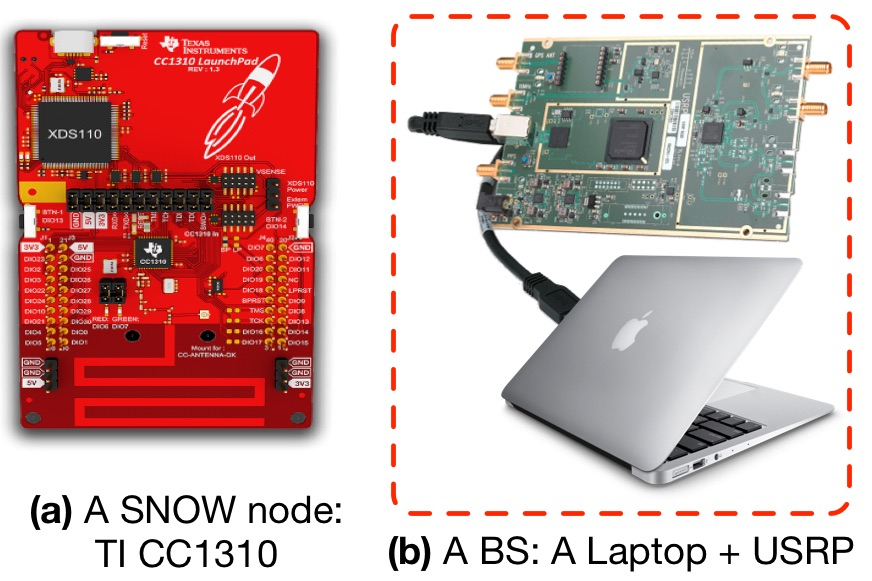
\includegraphics[width=0.34\textwidth]{figs/hardware.jpg}
%\vspace{-0.1in}
%\caption{\footnotesize SNOW Hardware.}
%\label{fig:hardware}
%\vspace{-0.1in}
%\end{figure} 


%We implemented SNOW on two hardware platforms -- USRP~\cite{usrp} using GNU radio~\cite{gnuradio} and TI CC1310~\cite{cc1310}. 
%Using a simple CSMA/CA based MAC protocol, our preliminary experiments showed its better scalability and energy efficiency over other LPWANs~\cite{snow, snow2, ton_snow}.  \revise{We observed a Tx range of 8km at 20dBm.}    
%CC1310 is a tiny, cheap ($<$\$30), and commercially off-the-shelf (COTS) device with a programmable PHY. 
%We implemented SNOW with CC1310 (using CC-ANTENNA-DK2)  as a SNOW node (Fig. \ref{fig:hardware} (a)) \cite{snowdemo}. The BS is a USRP210 with a laptop (Fig. \ref{fig:hardware} (b)). Since CC1310 allows us to use ASK modulation and up to 15dBm Tx power, we achieved 1.5km Tx range compared to 8km achieved using USRP. We have set a testbed using both USRP and CC1310 devices as SNOW nodes \cite{opensource}.  As the frequencies of SNOW's operating spectrum  are close to that (lower ISM band) of most LPWANs, its antenna form factor will be close to those in real production. 


\subsection{An Overview of LoRa}
\revise{Here we provide a brief overview of LoRa(Long-Range). Detailed description for the physical and link-layer of LoRa networks can be found in~\cite{LoRaWAN_spec_v1.1}. LoRa is the physical layer technology for an LPWAN. It's characteristics include extremely long-range which can be in the range of 3-7 miles depending on the environment and successful reception of packets even at extremely low signal-to-noise ratio. LoRa modulation is derived from \emph{Chirp Spread Spectrum (CSS)}. CSS modulation spreads the signal over the entire bandwidth, thus providing robustness to interference and enabling reception of packet at very low signal-to-noise ratio. The modulated signal consists of symbols/chirps, whose frequency linearly increases or decreases over time. Information is encoded onto each chirp using multiple cyclic shifted chips. The number of chips present in each symbol is controlled by the \emph{spreading factor}. Specifically, spreading factor is the ratio between symbol rate and chip rate. LoRa supports spreading factor in the range [6,12]. Spreading factor (SF) controls the data rate and thus the transmission time and energy consumption. A higher spreading factor reduces the data rate and thus increases the time on air for each packet leading to significant increase in energy consumption.  Transmissions on different spreading factors are orthogonal to each other. }

\revise{LoRa also supports different levels of forward error detection (FEC), called \emph{coding rates} in the range of $\frac{4}{5}$ to $\frac{4}{8}$ A higher coding rate provides resilience against bursts of interference, but increases the duration of each packet. Apart from coding rate and spreading factor, other configurable parameters for LoRa are carrier frequency, channel and bandwidth. Carrier frequency and channels vary from region to region depending on local regulation. For example, in the US band LoRa operates in the range 902-928MHz. For uplink communication in the US, there are 64 channels of bandwidth 125kHz and 8 channels of bandwidth 500kHz. For downlink, there are 8 channels of bandwidth 500kHz. }

\revise{The MAC protocol used with LoRa physical layer is called LoRa Wide Area Network(LoRaWAN). In LoRaWAN numerous nodes are directly connected to one of more gateways, which forward the data collected from nodes to a central network server. Thus, LoRa forms a star of star network topology. LoRaWAN supports classes of operation, namely class A,B and C. In all classes, nodes transmit using pure ALOHA. In class A, nodes transmit when they have data and open two receive windows after each transmission. In class B, gateway send periodic beacons to synchronize nodes. Between two beacons, the nodes wake up periodically to receive any packets from the gateway. In class C, the nodes are continuously listening for packets from the gateway.}
 
\subsection{System Model}
\revise{We consider LPWAN networks consisting of numerous nodes connected directly to one or more gateways. We consider a dense deployment where multiple LPWAN networks are operating in the same spectrum. We assume that the nodes and gateways of these networks do not posses any knowledge about each other and operate independently. Nodes are battery-powered and only wake-up if they have data to send. Nodes do not posses significant computing power and memory. Gateways are line-powered devices and are always active. We assume that the gateways can support concurrent receptions of multiple packets up to some limit. Thus, the gateways are limited by maximum number of simultaneous receptions $n$ which can be controlled by the network manager. If more than $n$ packets arrive at the gateway at the same time, some packets are dropped. Nodes rely on acknowledgements from the gateway to confirm successful reception of data. Nodes retransmit the packet if an acknowledgement is not received. The maximum number of retransmissions is also configured by the network manager.}